\documentclass[11pt, letterpaper]{article}

\usepackage[margin=2cm]{geometry}

\usepackage{color}
\definecolor{codegreen}{rgb}{0,0.6,0}
\definecolor{codegray}{rgb}{0.5,0.5,0.5}
\definecolor{codepurple}{rgb}{0.58,0,0.82}
\definecolor{backcolour}{rgb}{0.95,0.95,0.92}

\usepackage{listings}
\lstdefinestyle{mystyle}{
    backgroundcolor=\color{backcolour},
    commentstyle=\color{codegreen},
    keywordstyle=\color{magenta},
    numberstyle=\tiny\color{codegray},
    stringstyle=\color{codepurple},
    basicstyle=\footnotesize,
    breakatwhitespace=false,
    breaklines=true,
    captionpos=b,
    keepspaces=true,
    numbers=left,
    numbersep=5pt,
    showspaces=false,
    showstringspaces=false,
    showtabs=false,
    tabsize=2
}
\lstset{style=mystyle}

\usepackage{graphicx}
\usepackage{subcaption}
\usepackage{amsmath}
\usepackage[backend=biber]{biblatex} 
\addbibresource{references.bib} 
\usepackage[hidelinks]{hyperref}

%\DeclareMathOperator{\tr}{Tr}
\newcommand*{\op}[1]{\check{\mathbf#1}}
\newcommand{\bra}[1]{\langle #1 |}
\newcommand{\ket}[1]{| #1 \rangle}
\newcommand{\braket}[2]{\langle #1 | #2 \rangle}
\newcommand{\mean}[1]{\langle #1 \rangle}
\newcommand{\opvec}[1]{\check{\vec #1}}
\renewcommand{\sp}[1]{\begin{equation}\begin{split}#1\end{split}\end{equation}}


\newcommand*{\name}{Hussain Kitagawa}
\newcommand*{\mail}{h.kitagawa@studenti.unipi.it}
\newcommand*{\course}{Multimessenger Physics Laboratory}
\newcommand*{\teacher}{Barbara Patricelli, Massimiliano Razzano}
\newcommand*{\assignment}{April - May, 2023}

\begin{document}

\begin{flushleft}
    Name: \name \\
    E-mail: \mail\\
    Course: \course\\
    Teacher: \teacher\\
\end{flushleft}

\begin{center}
    \textbf{\large Gravitational Wave Data Analysis}\\
    \assignment 
\end{center}

\rule{\linewidth}{0.1mm}

\bigskip
\bigskip



%%%%%%%%%%%%%%%%%%%%
\section{Introduction of gravitational waves}
%%%%%%%%%%%%%%%%%%%%
\textbf{Introduction}\\
Gravitational waves are a phenomenon in which a space-time distortion generated by accelerated masses propagates at the speed of light. The gravitational wave is derived from the Einstein equation in general relativity, and its existence was predicted in 1916. The gravitational wave is generated through celestial phenomena,  such as black holes, neutron stars merger, and supernovas, and transmits its energy as electromagnetic radiation. A characteristic property of gravitational waves is their high permeability. Due to their properties, gravitational wave observations can provide information on the interior of high-density objects that do not emit electromagnetic waves, which cannot be obtained by conventional electromagnetic observations by telescope. However, since the typical amplitude of gravitational waves is about $~10^{-21}$, it has been required to have a high sensitivity for detecting the signal. Over a century since the anticipation of gravitational waves, the Laser Interferometer Gravitational-Wave Observatory (LIGO) accomplished direct measurement in 2015~\cite{Abbott_2016}. LIGO's twin detectors, located in Livingston and Hanford successfully detected gravitational waves originating from the merger of binary black holes~(GW150914). In addition, a notable result was obtained in 2017 with the detection of gravitational waves originating from the merger of binary neutron stars. This discovery was accompanied by comprehensive follow-up observations conducted across multiple wavelengths, such as gamma-ray, X-ray, infrared, and optical. This achievement heralded the emergence of a new field known as multimessenger astronomy.

\vskip\baselineskip
\textbf{\leftline{Detector principle}}\\
The LIGO detector is designed to detect the differential strain induced by gravitational waves. Its design is rooted in the fundamental principles of a Michelson interferometer, as shown in Figure~\ref{fig:ligo_interferometer}. The laser beam is directed towards the beam splitter, and the beam splitter's face is aligned at a 45-degree angle with respect to both the x-axis and the y-axis. The light propagates towards the mirrors positioned at the ends of the arms, where it undergoes reflection before returning to the beam splitter. When a gravitational wave traverses the detector, it causes elongation along the x-axis while inducing compression along the y-axis. Consequently, the effective path length within the arms is varied and the signal can be measured.

\begin{figure}[htbp]
  \centering
  \includegraphics[width=0.5\textwidth]{image/interferometer.png}
  \caption{A schematic view of LIGO detector~\cite{Abbott_2016}. The left top figure indicates the location of the LIGO detectors at Hanford and Livingston.}
  \label{fig:ligo_interferometer}
\end{figure}

%%%%%%%%%%%%%%%%%%%%
\section{Data analysis}
%%%%%%%%%%%%%%%%%%%%
The observed data obtained from the gravitational wave detector is typically contaminated with noise, posing difficulties in discerning true gravitational wave signals in the data. The analysis aims to investigate the presence of a signal in the data with backgrounds. The data collected between 2015 and 2017 at the LIGO observatory is used for the analysis. Specifically, gravitational wave emission generated during the coalescence of a binary black hole event~(GW150914) is analyzed. Finally, the mass and arrival time of gravitational waves is estimated. 

\vskip\baselineskip
\textbf{\leftline{Power spectral density~(PSD)}}\\
Assuming the instrumental noise in the random process timeseries x(t) can be expressed as probability density function $p_{X}(x)$. Considering the stationary process, the ensemble average~$\langle x \rangle$ is equivalent to the long time average and can be defined as,


\begin{equation}
\langle x \rangle := \int dx \, x \, p_X(x) = \lim_{{T \to \infty}} \int_{{-\frac{T}{2}}}^{{\frac{T}{2}}} dt x(t)
\end{equation}

where,
\begin{equation}
x_{T}(t) =
\begin{cases}
x(t) & \left(-\frac{T}{2} \leq t \leq \frac{T}{2}\right) \\
0 & \text{otherwise.}
\end{cases}
\end{equation}

The expected value of $x(t)^2$ is expressed as,
\begin{eqnarray}
\langle x^2 \rangle &=& \lim_{{T \to \infty}} \frac{1}{T} \int_{-\infty}^{\infty} dt {x^2}_{T}(t)\\
&=& \lim_{{T \to \infty}} \frac{2}{T} \int_{0}^{\infty} df\,|\,{\tilde{x}_{T}(f)}|^2\\
&=&\int_{0}^{\infty} df\, S_{x}(f).
\end{eqnarray}

Here in the second line, the Fourier transform of the time-limited function $\tilde{x}_{T}(f)$ is given as ${x^2}_{T}(t)$ from the Parseval's Theorem,

\begin{equation}
\int_{-\infty}^{\infty} dt \, |{{x}_{T}}(t)|^2  = \int_{-\infty}^{\infty} df\, |{{\tilde x}_{T}}(f)|^2.
\end{equation}

The power spectral density (PSD) for the given detector will be defined as,

\begin{eqnarray}
{S}_{x}(f) &:=& \lim_{{T \to \infty}} \frac{2}{T} |{{\tilde x}_{T}}(f)|^2\\
&=& \lim_{{T \to \infty}} \frac{2}{T} \int_{{-\frac{T}{2}}}^{{\frac{T}{2}}} dt x(t) e^{2\pi i f t}  \int_{{-\frac{T}{2}}}^{{\frac{T}{2}}} dt' x(t') e^{-2\pi i f t'}
\end{eqnarray}

The amplitude spectral density~(ASD) is obtained by taking the square root of PSD~\cite{Lecture_slide_2023}.

\vskip\baselineskip
\textbf{Amplitude spectral density and noise characterization}\\
The evolution of ASD is examined as a function of time series. The original data spans 1 hour, and a time interval spanning 30 minutes around the event is selected for the spectrum analysis. In order to check the time variation of ASD, the data is divided into a small time segment of 90 seconds~(a total of 20 data samples). The maximum and minimum ASD value at each frequency is obtained as shown in Figure~\ref{fig:ASD_time}. 





\begin{figure}[htbp]
  \centering
  \begin{subfigure}[b]{0.45\textwidth}
    \centering
    
\includegraphics[width=\textwidth]{image/L1_ASD_frequency.png}
    \caption{ASD for L1}
    \label{fig:figure1}
  \end{subfigure}
  \hfill
  \begin{subfigure}[b]{0.45\textwidth}
    \centering
    
\includegraphics[width=\textwidth]{image/H1_ASD_frequency.png}
    \caption{ASD for H1}
    \label{fig:figure2}
  \end{subfigure}
  \caption{The minimum and maximum value of ASD}
  \label{fig:ASD_time}
\end{figure}


The time dependency of the average value of ASD in a specific frequency region is also calculated. The average value of ASD between 50 and 100 Hz region is computed and compared with its standard deviation. The average value of ASD in each time segment~(90 seconds) varies within its standard deviation as shown in Figure~\ref{fig:ASD_average}. The ASD provides an indication of the sensitivity required for detecting gravitational wave signals. In the frequency range from 50 Hz to 100 Hz, both detectors reach a magnitude on the order of $10^{-23}$. The ASD values for the L1 detector vary over time series, whereas the ASD for the H1 detector remains stable throughout the entire period. The average ASD for H1 is slightly higher than that of L1, which indicates that the noise is relatively higher in H1.

\begin{figure}[htbp]
  \centering
  \begin{subfigure}[b]{0.45\textwidth}
    \centering
    
\includegraphics[width=\textwidth]{image/L1_ASD_average.png}
    \caption{ASD average for L1}
    \label{fig:figure1}
  \end{subfigure}
  \hfill
  \begin{subfigure}[b]{0.45\textwidth}
    \centering
    
\includegraphics[width=\textwidth]{image/H1_ASD_average.png}
    \caption{ASD average for H1}
    \label{fig:figure2}
  \end{subfigure}
  \caption{The blue line is the average value of ASD in the frequency band between 50 Hz to 100 Hz, which is calculated for each time interval~(90 seconds each). The red line represents the total average value of ASD for the whole data period in the frequency band between 50 Hz to 100 Hz and the green band is its standard deviation.}
  \label{fig:ASD_average}
\end{figure}


\vskip\baselineskip
\textbf{Quicklook time-domain analysis around the event}\\
To ensure that the acquired data corresponds to the operational period and covers the time span in which the event occurred, a basic data check is performed. The event that occurred in a valid DQ segment is shown in Figure~(\ref{fig:DQ1}, \ref{fig:DQ2}). The green band denotes the successful data which can be used for the analysis. A time interval of 20 seconds centered around the event is selected, as shown in Figure~(\ref{fig:strain_20_1}, \ref{fig:strain_20_2}). 
The band-pass filter between 64 to 300 Hz and a notch at 60 Hz are applied for L1 and H1. Figure~(\ref{fig:strain_filtered_1}, \ref{fig:strain_filtered_2}) shows after applying the filter, and the peak can be observed in the event with the high SNR around 2.4 seconds.

\begin{figure}[htbp]
  \centering

  
  \begin{subfigure}[b]{0.45\textwidth}
    \centering
    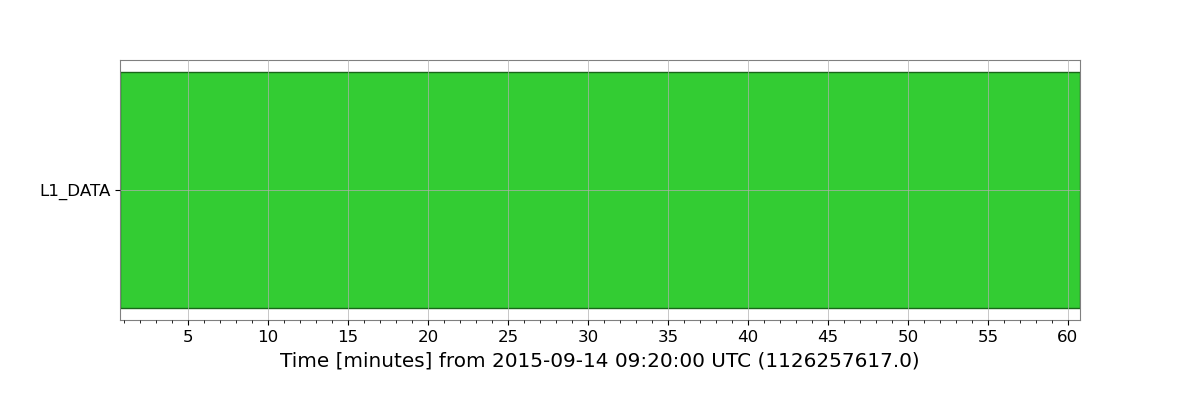
\includegraphics[width=\textwidth]{image/L1_data_green.png}
    \caption{L1 data}
    \label{fig:DQ1}
  \end{subfigure}
  \hfill
  \begin{subfigure}[b]{0.45\textwidth}
    \centering
    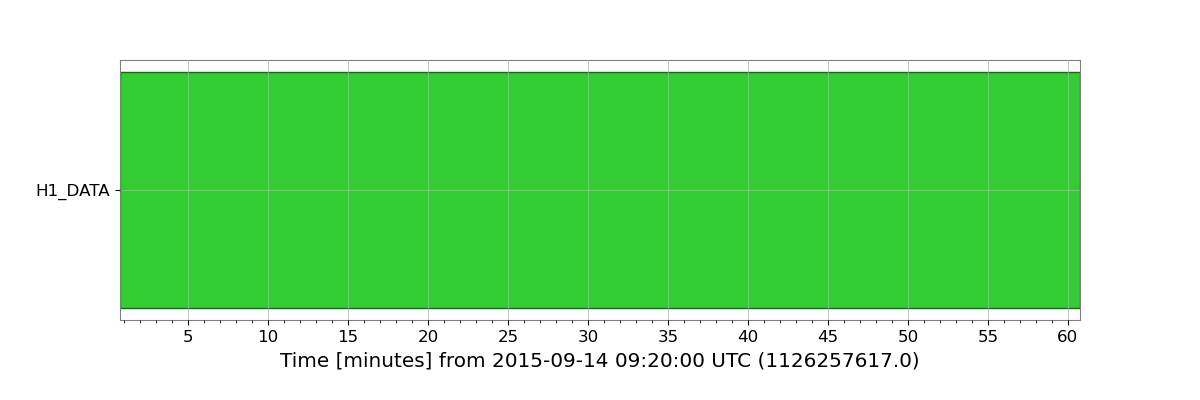
\includegraphics[width=\textwidth]{image/H1_data_green.png}
    \caption{H1 data}
    \label{fig:DQ2}
  \end{subfigure}

  
  \vspace{0.5cm}
  \begin{subfigure}[b]{0.45\textwidth}
    \centering
    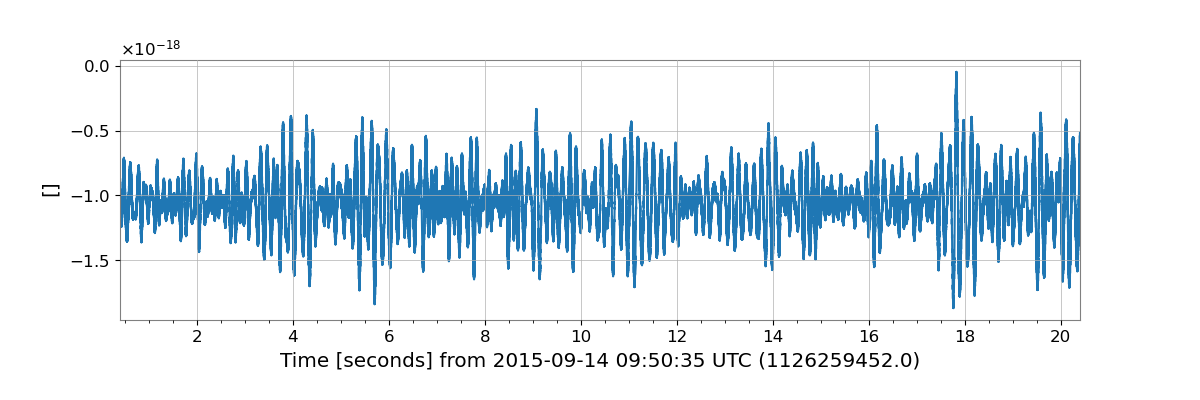
\includegraphics[width=\textwidth]{image/L1_data_20sec.png}
    \caption{L1 data with a time interval of 20 seconds around the event}
    \label{fig:strain_20_1}
  \end{subfigure}
  \hfill
  \begin{subfigure}[b]{0.45\textwidth}
    \centering
    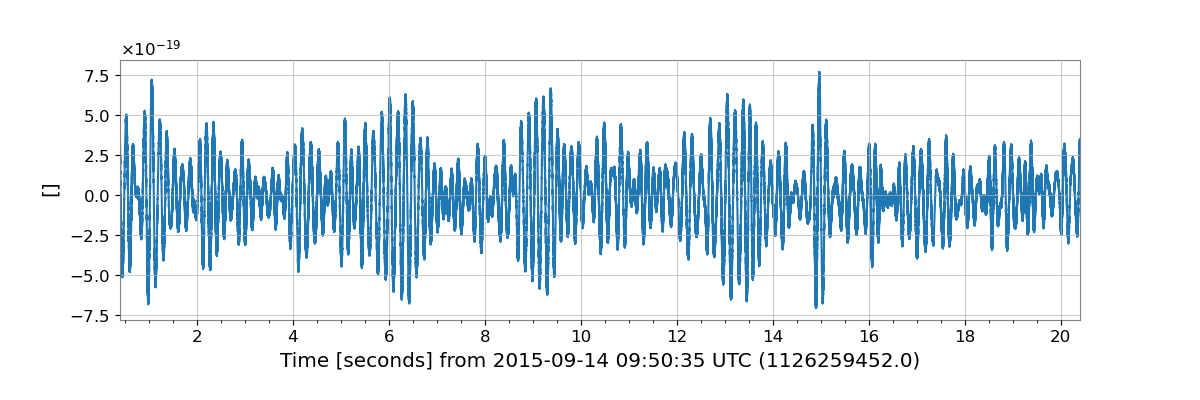
\includegraphics[width=\textwidth]{image/H1_data_20sec.png}
    \caption{H1 data with a time interval of 20 seconds around the event}
    \label{fig:strain_20_2}
  \end{subfigure}

 
  \vspace{0.5cm}
  \begin{subfigure}[b]{0.45\textwidth}
    \centering
    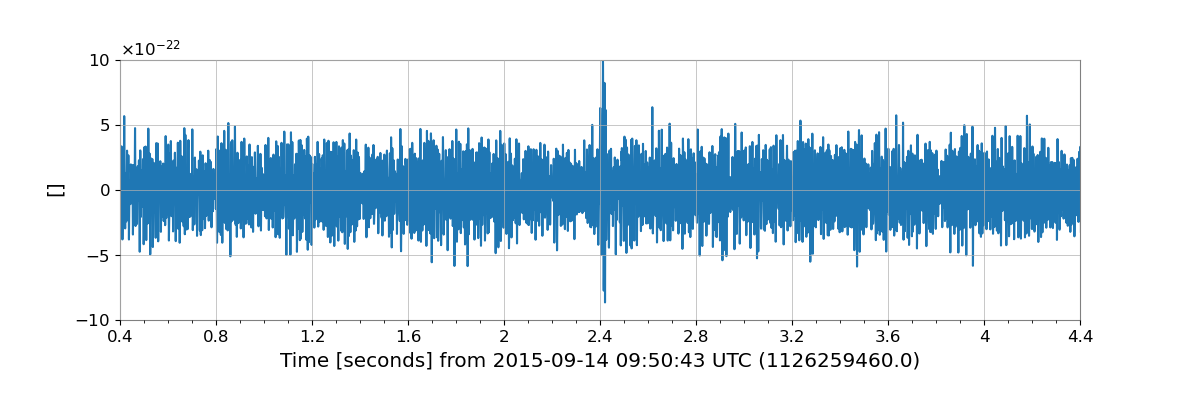
\includegraphics[width=\textwidth]{image/L1_data_filtered.png}
    \caption{L1 data after applying band-pass filtering}
    \label{fig:strain_filtered_1}
  \end{subfigure}
  \hfill
  \begin{subfigure}[b]{0.45\textwidth}
    \centering
    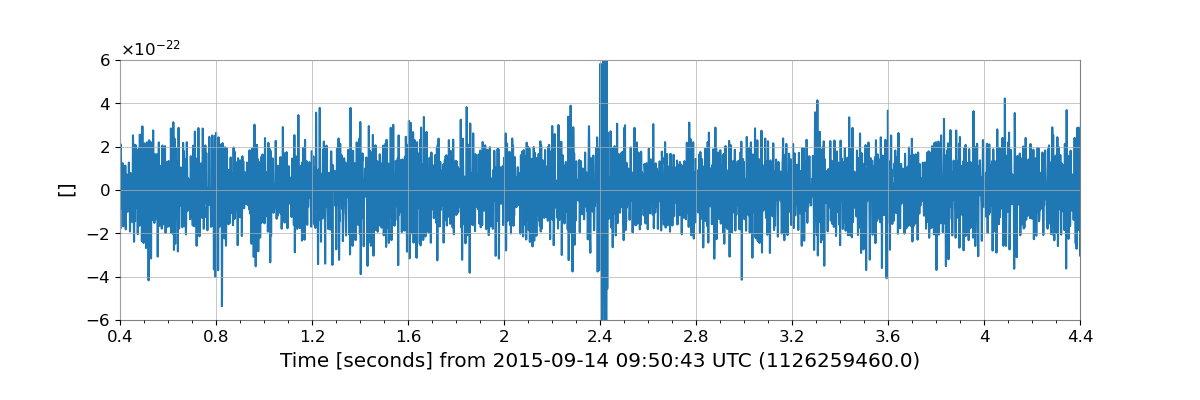
\includegraphics[width=\textwidth]{image/H1_data_filtered.png}
    \caption{H1 data after applying band-pass filtering}
    \label{fig:strain_filtered_2}
  \end{subfigure}

  
  \vspace{0.5cm}
  \begin{subfigure}[b]{0.45\textwidth}
    \centering
    
\includegraphics[width=\textwidth]{image/L1_data_filtered_2sec.png}
    \caption{L1 data after removing 2 seconds from the beginning and the end of the data}
    \label{fig:resampled_data_1}
  \end{subfigure}
  \hfill
  \begin{subfigure}[b]{0.45\textwidth}
    \centering
    
\includegraphics[width=\textwidth]{image/H1_data_filtered_2sec.png}
    \caption{H1 data after removing 2 seconds from the beginning and the end of the data}
    \label{fig:resampled_data_2}
  \end{subfigure}

  \caption{Quality check of the data for L1 and H1.}
  \label{fig:data_check}
\end{figure}




\vskip\baselineskip
\textbf{Signal search with template matching}\\
In this section, a signal processing method for analyzing raw time series data and searching for CBC signals using template matching is described.
In order to reduce the data size and computational cost, strain data is downsampled to the rate of 2048 Hz. The strain data resampled $\pm10$ seconds around the event after removing 2 seconds of data from both the beginning and end is shown in Figure~(\ref{fig:resampled_data_1}, \ref{fig:resampled_data_2}).

Using the resampling data, the maximum SNR for a gravitational wave signal can be estimated by creating a template bank of waveforms with various mass combinations of coalescence of two objects.
The analysis flow for the maximum SNR estimation is as follows:

\begin{itemize}
        \item Divide the data into 4 second segments and estimate the PSD for each. Then, interpolate it to match the frequency resolution of the data and exclude the data below 15 Hz as high-pass filtering
	\item  Generates a template bank of waveforms of a gravitational wave of non-rotating black holes over a combination of the mass of coalescence of two black holes~(m\_guess1 and m\_guess2)
        \item Apply PSD filtering and remove the initial and the final 4 seconds to account for the PSD
        \item Calculates the maximum SNR and its arrival time for L1 and H1
\end{itemize}

Here, the process iterates over each combination of m\_guess1 and m\_guess2~(solar mass), ranging from 25 to 35, with a mass step of 0.5. The maximum value of SNR for each combination is given in Figure~\ref{fig:m1_m2_grid}, and the arrival time for the highest SNR and its value with the set of m\_guess1 and m\_guess2 is obtained as ($\rm{SNR_{max}}$, m1, m2, time[sec]) = (13.3, 34.5, 34.5, 1126259462.418457) for L1 and ($\rm{SNR_{max}}$, m1, m2, time[sec]) = (19.5, 35.0, 35.0, 1126259462.425293) for H1 respectively. Based on the distance between L1 and H1~(3000 km), the expected arrival time differs by approximately 0.0031 seconds. The time difference could be caused by various factors: matching filters and modeling coalescing systems. Moreover, noise and its frequency band depend on its sources, such as the seismic motion of the Earth and instrumental noise. Further refinement of the filtering may enhance the SNR and result in more accurate arrival time measurements.

\begin{figure}[htbp]
  \centering
  \begin{subfigure}[b]{0.45\textwidth}
    \centering
    
\includegraphics[width=\textwidth]{image/L1_SNR_m1_m2.png}
    \caption{L1 data}
    \label{fig:figure1}
  \end{subfigure}
  \hfill
  \begin{subfigure}[b]{0.45\textwidth}
    \centering
    
\includegraphics[width=\textwidth]{image/H1_SNR_m1_m2.png}
    \caption{H1 data}
    \label{fig:figure2}
  \end{subfigure}
  \caption{The maximum values of the SNR in the m1 - m2 grid}
  \label{fig:m1_m2_grid}
\end{figure}

To align the template model with the data, the signal is shifted to the peak time, and the amplitude is rescaled according to the peak value. Finally, whiten method is applied to reduce noise in the time series data. Whiten method involves dividing the Fourier transform of the time series data by the ASD value of the noise. The inverse Fourier transform is applied to return the data back to the time domain. Once the data is whitened, a band-pass filter eliminates low-frequency and high-frequency noise components. Figure~\ref{fig:whiten} shows the result after the aforementioned process, where the H1 data is overlapped with the template model in the data period of 0.2 seconds before and 1 second after the coalescence time. The applied filtering includes high and low-frequency bandpass filtering and selects the data with frequencies within the range from 30 Hz to 300 Hz.

\begin{figure}[htbp]
  \centering
  \begin{subfigure}[b]{0.45\textwidth}
    \centering
    
\includegraphics[width=\textwidth]{image/L1_data_template.png}
    \caption{Template model for L1}
    \label{fig:figure1}
  \end{subfigure}
  \hfill
  \begin{subfigure}[b]{0.45\textwidth}
    \centering
    
\includegraphics[width=\textwidth]{image/H1_data_template.png}
    \caption{Template model for H1}
    \label{fig:figure2}
  \end{subfigure}
  \caption{Template model with the gravitational strain.}
  \label{fig:whiten}
\end{figure}


%Following the application of the bandpass filter, gravitational wave signals become discernible within the data.


%%%%%%%%%%%%%%%%%%%%
%\section{3}
%%%%%%%%%%%%%%%%%%%%
\newpage
\printbibliography
\textbf{Analysis codes}
\begin{itemize}
        \item experience---gw-data-analysis~\\(\url{https://github.com/hussainkitagawa/experience---gw-data-analysis.git})
        \item homework-01---data-input-output-with-python-hussainkitagawa~\\(\url{https://github.com/hussainkitagawa/homework-01---data-input-output-with-python-hussainkitagawa.git})
        \item homework-02---data-manipulation-with-pandas-hussainkitagawa~\\(\url{https://github.com/hussainkitagawa/homework-02---data-manipulation-with-pandas-hussainkitagawa.git})
        \item homework-03---basic-fitting-with-python-hussainkitagawa~\\(\url{https://github.com/hussainkitagawa/homework-03---basic-fitting-with-python-hussainkitagawa.git})
        \item homework-04---basics-of-object-oriented-programming-hussainkitagawa~\\(\url{https://github.com/hussainkitagawa/homework-04---basics-of-object-oriented-programming-hussainkitagawa.git})
\end{itemize}

\end{document}

